\documentclass{article}
\usepackage{graphicx} % Required for inserting images

\title{Parameter Estimation and Inverse Theory\\ Assignment 1}
\author{Parth Gupte}
\date{13th September 2023}

\begin{document}

\maketitle
\section{Q1}
\subsection{Experimental Procedure:}
In this experiment we generated:\\
\begin{enumerate}
    \item A random model with degree 3 and parameter values between -10 and 10.
    \item 20 random data points from this model with range of x values in -10 and 10 and y values having 10\% Gaussian noise.
\end{enumerate}
We then estimate an L2 model that fits these data points.\\

\subsection{Outcomes:}
\begin{enumerate}
    \item Estimated and True Parameter table (increasing order of degree):\\
    \\
    \begin{tabular}{|c|c|} 
        \hline 
       True Model & Estimated Model\\ 
       \hline 
       0.9762700785464951 & 0.21448703477967523\\ 
       \hline 
       4.30378732744839 & 7.197065172027351\\ 
       \hline 
       2.055267521432878 & 1.8190459732807414\\ 
       \hline 
       0.8976636599379368 & 0.8935207167011852\\ 
       \hline 
    \end{tabular}
\clearpage
    \item Curve fitting plot:\\
    \begin{figure}[h]
        \centering
        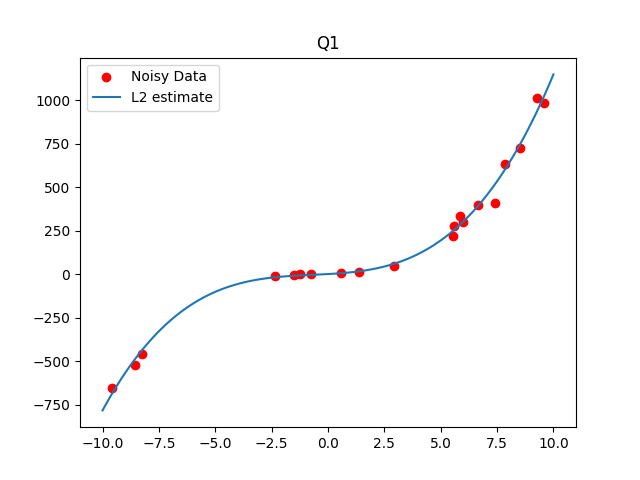
\includegraphics[width = 15 cm]{figs/Q1plot.png}
        \caption{L2 fit with noisy data}
    \end{figure}
\clearpage
    \item Data Resolution Matrix Image:
    \begin{figure}[h]
        \centering
        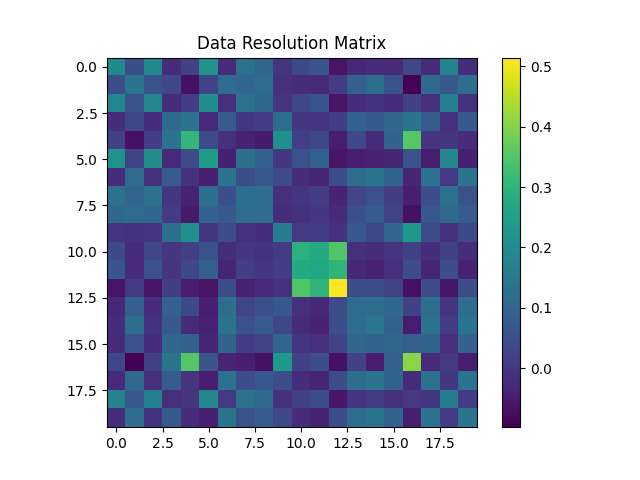
\includegraphics[width = 15 cm]{figs/Q1dataresmtrix.png}
        \caption{Data Resolution Matrix}
    \end{figure}
\clearpage
    \item Model Resolution Matrix:
    \begin{figure}[h]
        \centering
        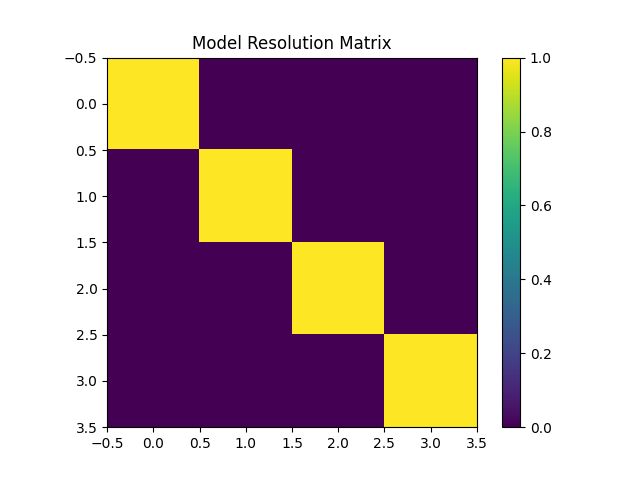
\includegraphics[width = 15 cm]{figs/Q1modelresmatrix.png}
        \caption{Model Resolution Matrix}
    \end{figure}
\clearpage
\end{enumerate}

\subsection{Observations:}
\begin{enumerate}
    \item The L2 norm solution fits well to the noisy data.
    \item The Model resolution matrix is nearly the identity matrix, that means the estimated model is very close to the real model.
\end{enumerate}

\section{Q2}
\subsection{Experimental Procedure:}

In this experiment we:
\begin{enumerate}
    \item Skewed the y value of one of the points to make it an outlier.
    \item Estimated an L1 model for the data (tolerance = 0.5).
    \item Estimated an L2 model for the data.
\end{enumerate}

\subsection{Outcomes:}

\begin{enumerate}
    \item Estimated and True Parameter values (increasing order of degree):\\\\
    \begin{tabular}{|c|c|c|} 
        \hline 
       True Model & L1 Estimated Model & L2 Estimated Model\\ 
       \hline 
       0.9762700785464951 & 14.283590517938137 & 75.78986897228734\\ 
       \hline 
       4.30378732744839 & 4.568483171751723 & -9.386595257710752\\ 
       \hline 
       2.055267521432878 & 1.9189171649341006 & 0.9148557125311957\\ 
       \hline 
       0.8976636599379368 & 0.8946313395790639 & 1.1023668406951843\\ 
       \hline 
       \end{tabular}
\clearpage
       \item Curve fitting plot:
       \begin{figure}[h]
            \centering
            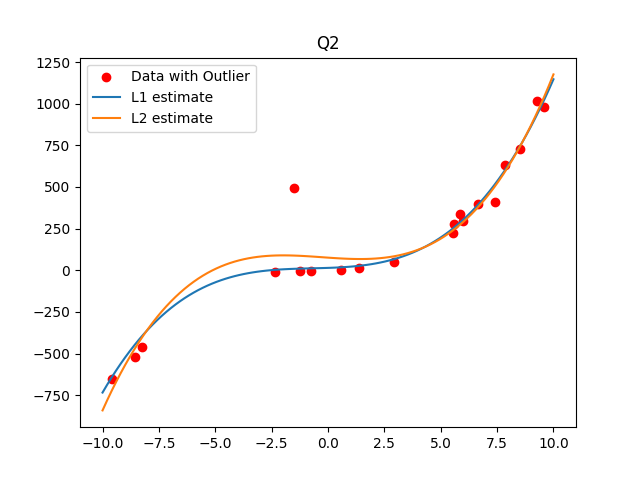
\includegraphics[width = 15 cm]{figs/Q2plots.png}
        \caption{Comaparison of L1 and L2 estimate}
    \end{figure}
\clearpage
        \item Curves at each iteration
        \begin{figure}[h]
            \centering
            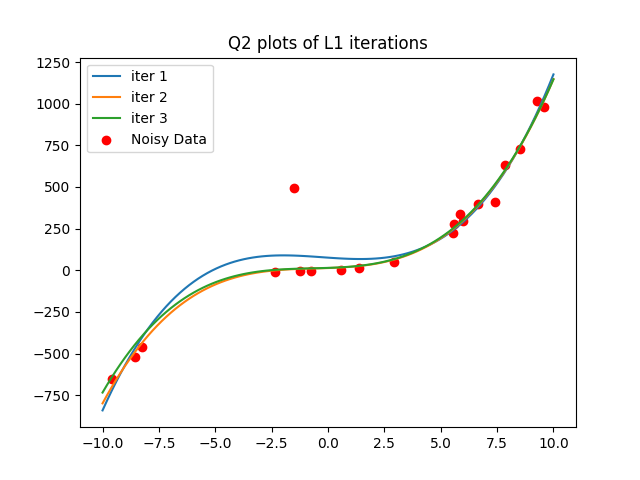
\includegraphics[width = 15 cm]{figs/L1iterplot.png}
        \caption{Plots at each iteration}
    \end{figure}
\clearpage
\end{enumerate}

\subsection{Observations:}
\begin{enumerate}
    \item L2 model performs worse than L1 on data with an outlier.
    \item L1 model converges to an accurate solution fairly quickly.
    \item L1 model is not very affected by the outlier data point but L2 is.
\end{enumerate}

\section{Q3}
\subsection{Experimental Procedure:}
In this experiment we used constraint optimization techinques to fit a 3 degree polynomial to the data such that it passes through 2 of the randomly choosen points perfectly.\\

\subsection{Outcomes:}
\begin{enumerate}
    \item Estimated and True Parameter Values (increasing order of degree):\\
    \\
    \begin{tabular}{|c|c|} 
        \hline 
       True Model & Estimated Model\\ 
       \hline 
       0.9762700785464951 & -2.8436627173615534\\ 
       \hline 
       4.30378732744839 & -0.6246210348928685\\ 
       \hline 
       2.055267521432878 & 1.8487298229849463\\ 
       \hline 
       0.8976636599379368 & 0.9908810802375109\\ 
       \hline 
    \end{tabular}
\clearpage
    \item Curve fitting plot:\\
    \begin{figure}[h]
        \centering
        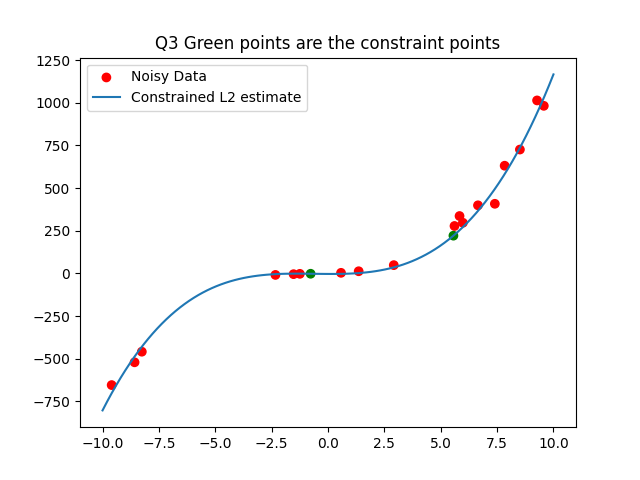
\includegraphics[width = 15 cm]{figs/Q3plots.png}
    \caption{Constrained fit}
\end{figure}
\end{enumerate}

\subsection{Observations:}
\begin{enumerate}
    \item The curve passes perfectly through the constraint points.
\end{enumerate}

\section{Python Code:}
\begin{verbatim}
import numpy as np
import matplotlib.pyplot as plt
import csv
import random as rd

def generate_random_model(deg:int,rng:tuple):
    '''
    Enter a degree and a range and a model is generated for that range and degree
    '''
    m = np.random.uniform(low = rng[0], high = rng[1], size = (deg+1,1))
    return m

def gen_random_data(model:np.ndarray,size = 20, noise = 0.1,rng = (-10,10)):
    '''
    Enter a model, and data is generated for that model with added guassian noise
    '''
    f_0 = np.random.uniform(low = rng[0], high = rng[1], size = (size,1))
    F = np.concatenate([f_0**i for i in range(len(m))], axis=1)
    d_true = np.matmul(F,m) 
    d = d_true + noise*d_true*np.random.normal(0,1,d_true.shape)
    return F,d

def L2_norm(V:np.ndarray):
    S = (sum(V**2)/len(V))**(1/2)
    return S

def estimate_model_L2(F:np.ndarray,d:np.ndarray):
    '''
    Estimates the model using L2 norm minimisation formula for full coloumn rank matrices
    '''
    m_est = np.matmul(np.matmul(np.linalg.inv(np.matmul(F.transpose(),F)),F.transpose()),d)
    return m_est

def estimate_model_L1(F:np.ndarray,d:np.ndarray,t_0):
    '''
    Estimates the model using L1 norm minimisation algorithm
    '''
    m_L = []
    u = 1
    F_og, d_og = F.copy(), d.copy()
    while True:
        m = estimate_model_L2(F,d)
        plot_model(m,"iter "+str(u))
        m_L.append(m)
        if len(m_L) >2:
            del m_L[0]
        if len(m_L) == 2:
            t = L2_norm(m_L[1]-m_L[0])/(1+L2_norm(m_L[1]))
            if t<t_0:
                break
        r = d - np.matmul(F,m)
        R = np.zeros((r.shape[0],r.shape[0]))
        # print(F.transpose().shape,R.shape,d.shape)
        for i in range(r.shape[0]):
            R[i,i] = 1/abs(r[i][0])
        F, d = np.matmul(np.matmul(F.transpose(),R),F), np.matmul(np.matmul(F.transpose(),R),d)
        u += 1
    plot_data(F_og,d_og)
    plt.legend()
    plt.title("Q2 plots of L1 iterations")
    # plt.savefig("assignment1/figs/L1iterplot.png")
    plt.show()
    return m

def F_dagger_L2(F:np.ndarray):
    return np.matmul(np.linalg.inv(np.matmul(F.transpose(),F)),F.transpose())

def numpy_to_csv(arr:np.ndarray):
    f = open("assignment1//model_table.csv","w")
    writer = csv.writer(f)
    writer.writerow(["True Model","Estimated Model"])
    for i in range(arr.shape[0]):
        row = arr[i]
        writer.writerow(row)
    f.close()


def numpy_to_csv_Q2(arr:np.ndarray):
    f = open("assignment1//model_table_Q2.csv","w")
    writer = csv.writer(f)
    writer.writerow(["True Model","L1 Estimated Model", "L2 Estimated Model"])
    for i in range(arr.shape[0]):
        row = arr[i]
        writer.writerow(row)
    f.close()


def numpy_to_csv_Q3(arr:np.ndarray):
    f = open("assignment1//model_table_Q3.csv","w")
    writer = csv.writer(f)
    writer.writerow(["True Model","Estimated Model"])
    for i in range(arr.shape[0]):
        row = arr[i]
        writer.writerow(row)
    f.close()

def plot_model(m:np.ndarray,label:str):
    P = list(m.transpose()[0])
    P.reverse()
    poly_obj = np.poly1d(P)
    X = np.linspace(-10,10,100)
    plt.plot(X,poly_obj(X),label = label)   

def plot_data(F,d,label = 'Noisy Data'):
    plt.scatter(list(F[:,1]),list(d),color = 'r',label = label)    

def plot_data_Q3(F,d,L,label = 'Noisy Data'):
    colors = ['r']*F.shape[0]
    for i in L:
        colors[i] = 'g'
    plt.scatter(list(F[:,1]),list(d),c = colors,label = label)    

def matrix_img(M:np.ndarray,title:str):
    plt.imshow(M)
    plt.title(title)
    plt.colorbar()



np.random.seed(0)
#Q1
m = generate_random_model(3,(-10,10)) # generated a random model
F, d = gen_random_data(m) #generate random data with noise for said model
m_est = estimate_model_L2(F,d) #estimate model from data
plot_data(F,d)
plot_model(m_est,"L2 estimate")
plt.legend()
plt.title("Q1")
# plt.savefig("assignment1/figs/Q1plot.png")
plt.show()


F_dggr = F_dagger_L2(F)
data_res_matrix = np.matmul(F,F_dggr)
matrix_img(data_res_matrix,"Data Resolution Matrix")
# plt.savefig("assignment1/figs/Q1dataresmtrix.png")
plt.show()

model_res_matrix = np.matmul(F_dggr,F)
matrix_img(model_res_matrix, "Model Resolution Matrix")
# plt.savefig("assignment1/figs/Q1modelresmatrix.png")
plt.show()

#save model values
M = np.concatenate((m,m_est),axis=1)
numpy_to_csv(M)

#Q2
d_copy = d.copy()
d_copy[0] += 500 # adding outlier
m_est_L1 = estimate_model_L1(F,d_copy,0.5)
m_est_L2 = estimate_model_L2(F,d_copy)
plot_data(F,d_copy,"Data with Outlier")
plot_model(m_est_L1,"L1 estimate")
plot_model(m_est_L2,"L2 estimate")
plt.legend()
plt.title("Q2")
# plt.savefig("assignment1/figs/Q2plots.png")
plt.show()

#save model values
numpy_to_csv_Q2(np.concatenate((m,m_est_L1,m_est_L2),axis=1))

#Q3

no_of_const_pts = 2
p,q = F.shape
idx_F = list(range(p))
L = list(np.random.choice(idx_F,no_of_const_pts))
G = F[L]
h = d[L]
not_L = []
for x in idx_F:
    if x not in L:
        not_L.append(x)
G_0 = F[not_L]
d_0 = d[not_L]
G_0TG_0 = np.matmul(G_0.transpose(),G_0)
GT = G.transpose()

k = G_0.shape[1]
l = G.shape[0]
A = np.zeros((k+l,k+l))
A[:k,:k] = G_0TG_0
A[:k,k:] = GT
A[k:,:k] = G

G_0Td_0 = np.matmul(G_0.transpose(),d_0)

Y = np.zeros((k+l,1))
Y[:k] = G_0Td_0
Y[k:] = h

m_contr_est = np.matmul(np.linalg.inv(A),Y)[:k]

plot_data_Q3(F,d,L)
plot_model(m_contr_est,"Constrained L2 estimate")
plt.legend()
plt.title("Q3 Green points are the constraint points")
# plt.savefig("assignment1/figs/Q3plots.png")
plt.show()

#save model values
numpy_to_csv_Q3(np.concatenate((m,m_contr_est),axis=1))





\end{verbatim}




\end{document}
